\chapter{Aufbau eines künstlichen neuronalen Netzes}
Im Nachfolgenden wird der allgemeine Aufbau eines einfachen Neuronalen Netzes in Python erklärt. Dazu wird ein Netzwerk ohne versteckte Schichten und drei Trainingswerten verwendet. Im Anschluss wird die Erweiterung des Netzwerkes mit mehreren versteckten Schichten erläutert. Weiterhin wird das eingesetzte Gradientenverfahren zur Reduzierung des Fehlers im Netz erläutert.


\section{Allgemeine Struktur des neuronalen Netzes}
Der grundlegende Aufbau des eingesetzten backpropagation Netzes soll im Folgenden an einem vereinfachten Netz ohne versteckte Schichten verdeutlicht werden. Zum Einsatz kommt neben \emph{Python 2.7} die Erweiterung \emph{NumPy} zur Unterstützung von mehrdimensionalen Arrays und Matrizen.
 
Für die Veranschaulichung soll die Ausgabe anhand der drei Eingabespalten vorhergesagt werden \tabref{sampledata}. Jede Spalte steht für einen Eingabeknoten des Netzwerkes mit jeweils vier Trainingsdaten.

\begin{table}[h!]
	\centering	
	\begin{tabular}{c|c|c|c}
	  \multicolumn{3}{c|}{\textbf{Eingabe}} & \textbf{Ausgabe} \\ \hline 
    0 & 0 & 1 & 0 \\ \hline
    1 & 1 & 1 & 1 \\ \hline
    1 & 0 & 1 & 1 \\ \hline
    0 & 1 & 1 & 0 \\ \hline
	\end{tabular}
	\caption{Ein- und Ausgabe für das Netz}
	\label{sampledata}
\end{table}

Die eingesetzte Aktivierungsfunktion ist eine Sigmoid-Funktion \lstref{sigmoidcode} mit der sich ebenfalls die Ableitung bzw. Steigung des jeweiligen Wertes berechnen lässt.

\begin{lstlisting}[caption={Sigmoid-Funktion}, label={sigmoidcode}]
def sigmoid(x, deriv = False):
    if(deriv == True):
        return x*(1-x)
    return 1/(1+np.exp(-x))
\end{lstlisting}

Die Ein- und Ausgabedaten werden in NumPy Arrays \emph{X} und \emph{Y} hinterlegt in denen jede Reihe ein Trainingsdatensatz darstellt. Die Werte für die Gewichte \emph{syn0} werden zufällig über einen Seed initialisiert \lstref{initgewicht}. So lässt sich bei mehrfacher Ausführung ein deterministisches Verhalten produzieren um eine Vergleichbarkeit zu gewährleisten. Da bei diesem Beispiel nur zwei Schichten (Ein- und Ausgabe) zum Einsatz kommen wird nur eine Gewichtsmatrix benötigt um diese beiden Schichten miteinander zu verbinden. Die Dimension dieser Matrix wird von dem Verhältnis der Ein- und Ausgaben, also 3:1, festgelegt.

\begin{lstlisting}[caption={Initialisierung Gewichte}, label={initgewicht}]
syn0 = 2*np.random.random((3, 1)) - 1
\end{lstlisting}

Der Lernprozess wird beispielhaft über zehntausend Durchläufe vorgenommen \lstref{lernprozess}. Das Netz besteht aus den zwei Schichten \emph{l0} und \emph{l1}. Die Eingabedaten werden direkt an die erste Schicht \emph{l0} übergeben. Dabei werden alle vier Trainingsdaten auf einmal verarbeitet (Full-Batch). In der zweiten Schicht \emph{l1} wird versucht die Ausgabe in der ersten Iteration direkt vorherzusagen (Zeile 3). Dabei wird die Eingabematrix \emph{l0} mit der Gewichtsmatrix \emph{syn0} multipliziert. Das Ergebnis wird anschließend an die Sigmoid Funktion übergeben. Bei vier Trainingsdaten erhält man so vier Vorhersagen für die gesuchte Ausgangsbelegung. Jeden Ausgabe stellt dabei den Versuch des Netzes dar anhand der Eingabedaten eine korrekte Vorhersage zu treffen.

\begin{lstlisting}[caption={Lernprozess},label={lernprozess}]
for iter in xrange(10000):
    l0 = X
    l1 = sigmoid(np.dot(l0, syn0))
    l1_error = y - l1
    l1_delta = l1_error * sigmoid(l1, True)
    syn0 += np.dot(l0.T, l1_delta)
\end{lstlisting}    

In Zeile 4 lässt sich die Vorhersage mit dem tatsächlichen Ergebnis vergleichen und der Fehler berechnen. Im der nächsten Zeile wird unter Zuhilfenahme der Ableitung der Sigmoid-Funktion \imgref{derivesigmoid} bestimmt, wie zuversichtlich das Netzwerk für diesen Wert ist. Das Ziel ist es dabei den Fehler für Werte zu reduzieren bei denen sich das Netz sehr sicher ist. Je geringer die Steigung in einem Punkt (grüne und violette Steigung), umso zuversichtlicher ist das Netz entweder eine richtige, oder falsche Aussage getroffen zu haben. Bei unsicheren Vorhersagen ist der Wert der Steigung am größten und dadurch werden diese Fehler für die nächste Iteration am stärksten berücksichtigt.

\begin{figure}[h!]
	\begin{center}
	\fbox{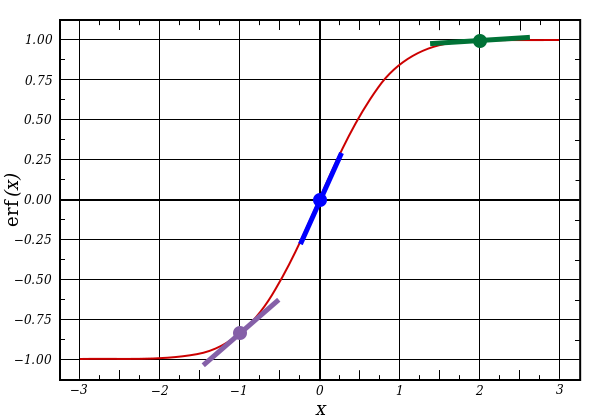
\includegraphics[width=0.9\textwidth]{pictures/sigmoid-deriv.png}}
	\caption{Ableitung Sigmoid-Funktion}
	\label{derivesigmoid}
	\end{center}
\end{figure}

Im letzten Schritt (Zeile 6) werden die Gewichte mit dem entsprechend berechneten Fehlern aktualisiert und der Prozess beginnt von neuem.

\newpage

\section{Gradientenverfahren}
\label{chap_gradient}
Zur Optimierung des neuronalen Netzes wird das Gradientenverfahren eingesetzt \imgref{gradient}. Ziel dieses Verfahrens ist es, ein lokales Minimum zu finden. Dabei wird die Steigung an der aktuellen Position berechnet und anhand des Vorzeichens entschieden ob sich die nächste Position rechts oder links von der aktuellen Stelle befinden soll. Bei einem negativen Vorzeichen ist die Richtung rechts, bei einem positiven links. Dieser Vorgang wird solange wiederholt, bis die Steigung in einem Punkt den Wert \emph{0}, oder ein bestimmten vorgegebenen Wert, erreicht.

\begin{figure}[h!]
	\begin{center}
	\fbox{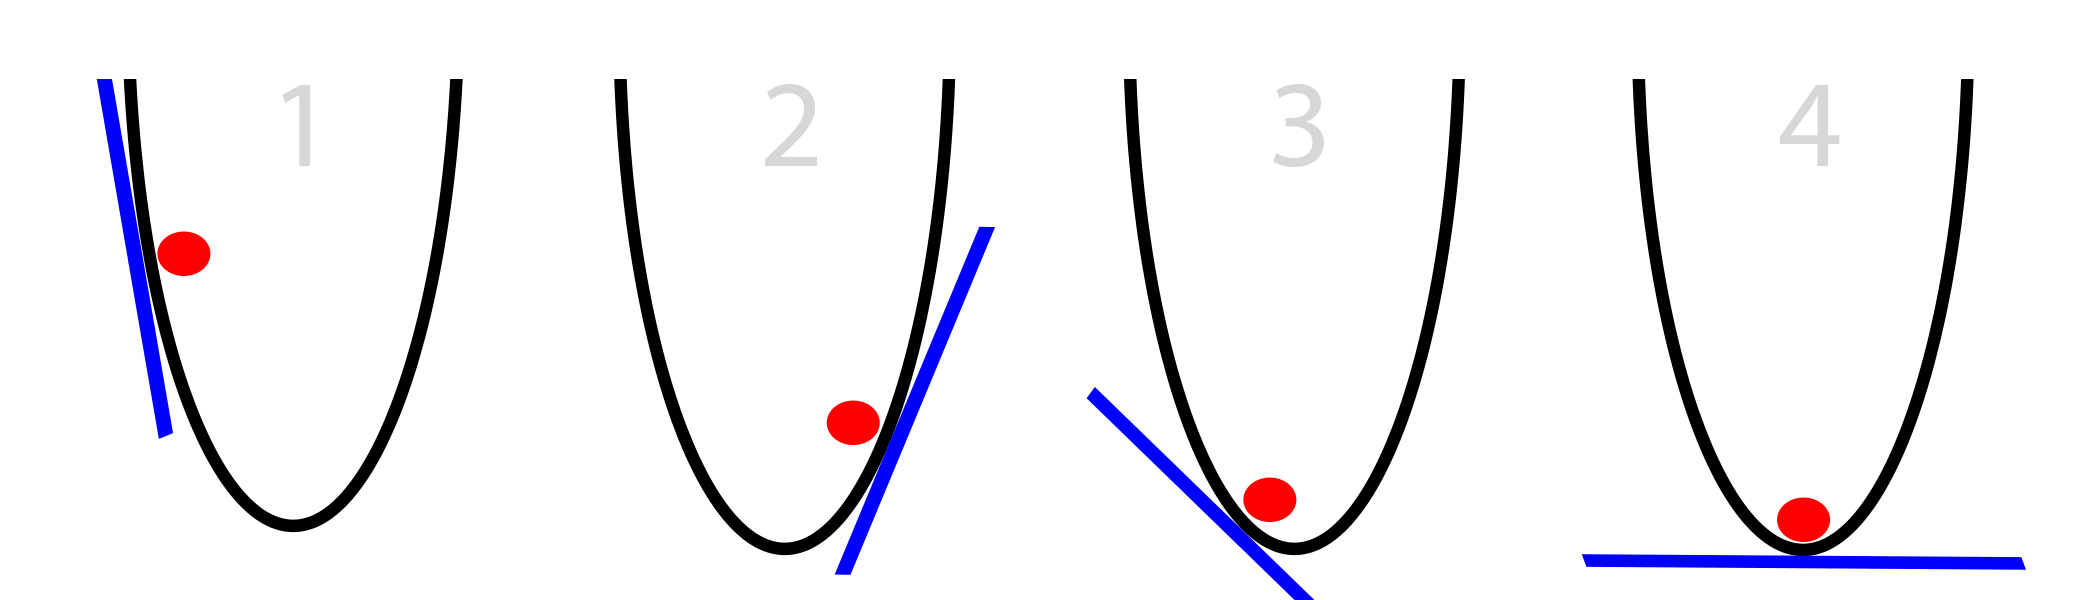
\includegraphics[width=0.9\textwidth]{pictures/sgd_optimal.png}}
	\caption{Gradientenverfahren}
	\label{gradient}
	\end{center}
\end{figure}

Die Schwierigkeit besteht darin, einen geeigneten Faktor zu bestimmen um den die Position geändert wird. Ein einfacher Ansatz ist dabei, die Verschiebung anhand der Steigung zu bestimmen. Je größer der Wert einer positiven Steigung, desto weiter wird die Position nach links verschoben. Je kleiner der Wert umso geringer fällt die Richtungsänderung aus. So werden Änderungen geringer bei einer Annäherung an ein lokales Minimum. Sollte der Nullpunkt erreicht werden, konvergiert das Verfahren. Bei zu großen Richtungsänderungen kann das Verfahren divergieren und man entfernt sich immer weiter von dem gesuchten Minimum.

Um dies zu verhindern wird ein \emph{Alpha} Wert eingeführt. Der Wertebereich von \emph{Alpha} liegt zwischen 0 und 1. Die neue Position wird nun durch den alten Positionswert und dem Produkt aus Steigung und Alphawert ermittelt. Bei der Wahl eines geeigneten Alphawertes muss berücksichtigt werden, dass ein zu kleiner Wert das Gradientenverfahren ausbremst und ein zu großer Wert den Einfluss auf das Ergebniss minimiert oder das Verfahren divergieren lässt.

\begin{figure}[h!]
	\begin{center}
	\fbox{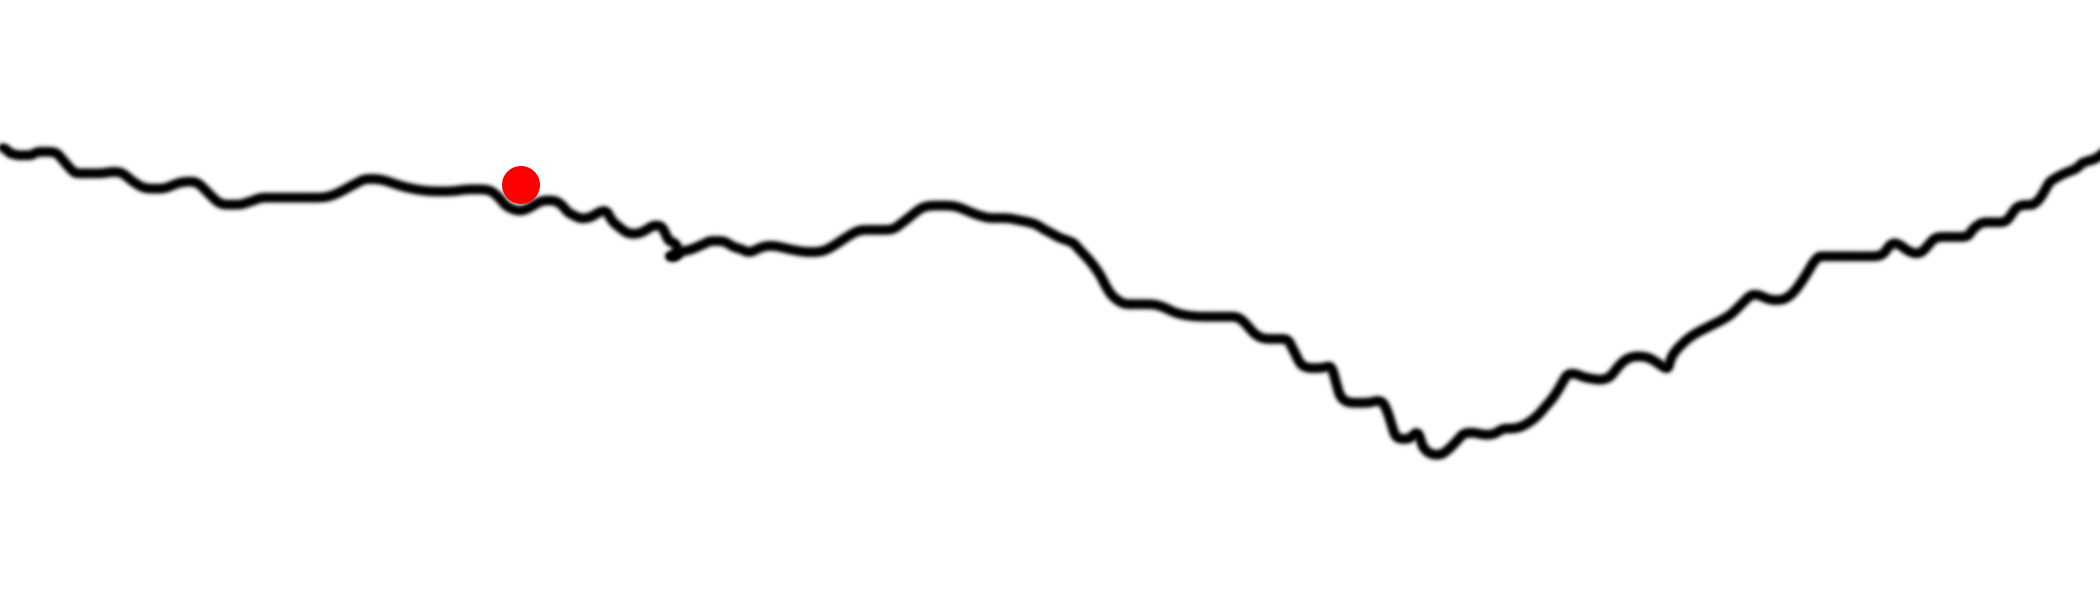
\includegraphics[width=0.7\textwidth]{pictures/alpha_small1.png}}
	\caption{Alphawert Einfluss (Teil 1)}
	\label{alpha1}
	\end{center}
\end{figure}

Die Wahl eines zu geringen Alphawertes kann zu zwei Problemen führen. Zum einen kann das Verfahren sich in lokalen Minima festsetzen \imgref{alpha1}, sodass das eigentliche Minimum des zu untersuchenden Abschnittes nicht gefunden wird. Im zweiten Fall \imgref{alpha2} fallen die Änderungen bedingt durch ein zu kleines \emph{Alpha} so gering aus, dass sich die Laufzeit zum Auffinden des Minimums enorm steigert.

\begin{figure}[h!]
	\begin{center}
	\fbox{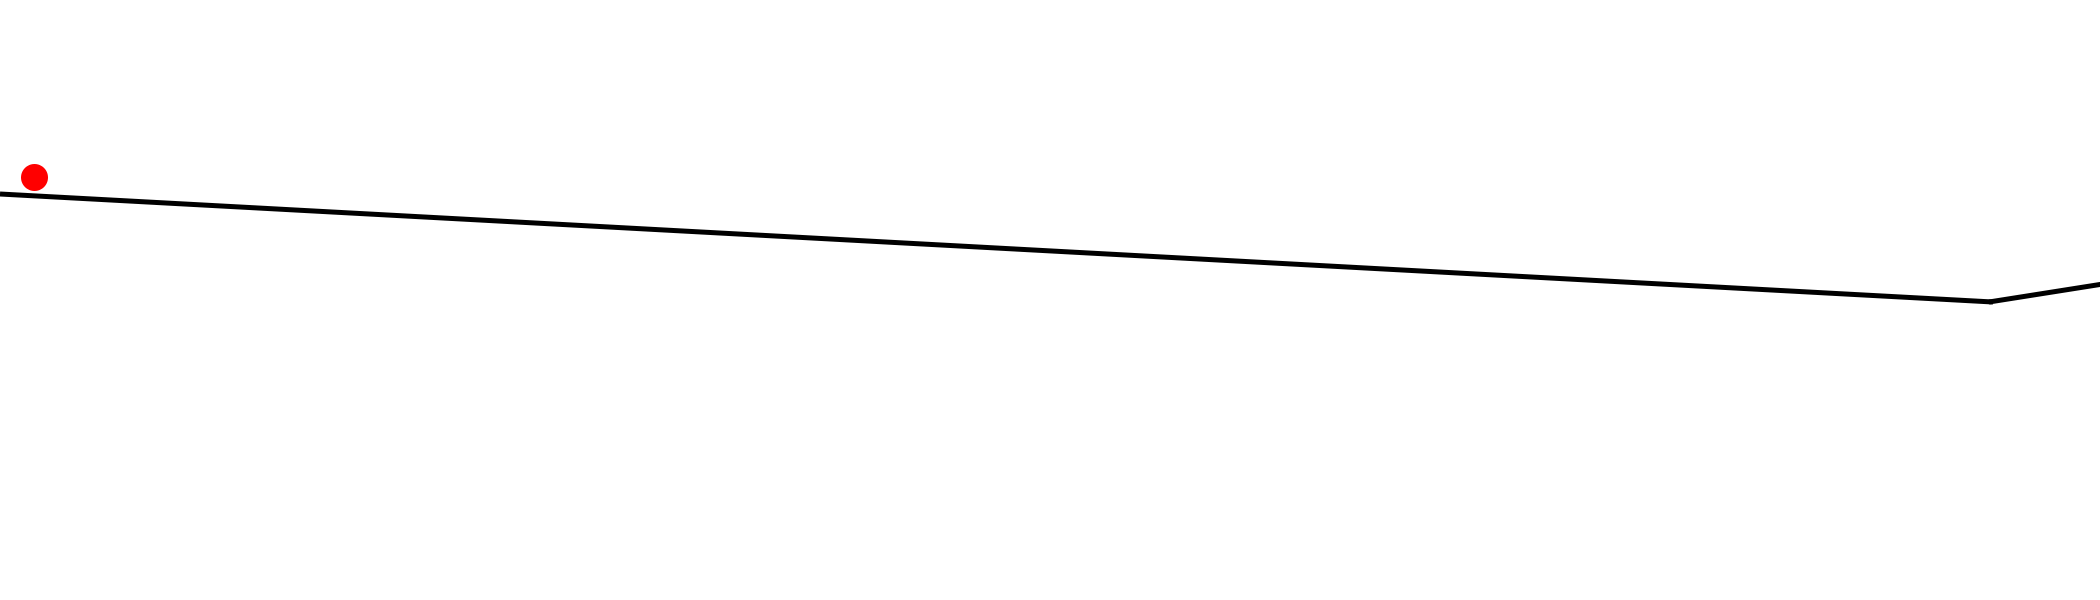
\includegraphics[width=0.7\textwidth]{pictures/alpha_small2.png}}
	\caption{Alphawert Einfluss (Teil 2)}
	\label{alpha2}
	\end{center}
\end{figure}


\newpage
\section{Erweiterung des Netzwerkes}
Durch eine Erweiterung des Netzwerkes mit mehreren versteckten Schichten und Neuronen steigt die Leistungsfähigkeit, wodurch eine Kapselung von Funktionen notwendig wird um die Übersicht und Einfachheit weiterhin zu gewährleisten. Im Folgenden werden die einzelnen Funktionen zur Inbetriebnahme des Netzes erläutert.

Das Netzwerk lässt sich durch Parameterübergabe an die Initialisierungsfunktion \lstref{init} mit einer beliebigen Anzahl von versteckten Schichten und Neuronen erstellen. Die Ein- und Ausgabeschicht wird dabei auf die entsprechenden Größen der Trainings- und Ausgabedaten angepasst. Die Gewichte werden mit zufälligen Werten vorbesetzt, wobei immer derselbe Seed zum Einsatz kommt (Zeile 2) um eine Vergleichbarkeit zu erreichen, die zwischen verschiedenen Durchgängen nur von der Anzahl der Schichten und Neuronen abhängig ist.

\begin{lstlisting}[caption={Initialisierung des Netzes},label={init}]
def initNetwork(inputArraySize, outputArraySize, hiddenLayerCount, hiddenLayerSize):
    np.random.seed(1)
    syns = []
    syns.append(2*np.random.random((inputArraySize, hiddenLayerSize)) - 1)
    for i in range(hiddenLayerCount):
        syns.append(2*np.random.random((hiddenLayerSize,hiddenLayerSize)) - 1)
    syns.append(2*np.random.random((hiddenLayerSize,outputArraySize)) - 1)
    return syns
\end{lstlisting}        

Nachdem das Netzwerk durch die Init-Funktion erstellt wurde, kann der Trainingsvorgang begonnen \lstref{train} werden. Dafür werden neben den Trainingsdaten (\texttt{inputData} und \texttt{outputData}) Vorgaben für den Fehlerwert und die Rundenzahl benötigt. Durch diese beiden Parameter lassen sich die Abbruchbedingungen des Netzes festlegen. Diese ist entweder erreicht wenn die maximale Anzahl an Trainingsrunden erreicht wurde oder der Fehlerwert das vorgegebene Minimum erreicht hat (Zeile 3). Eine Reduzierung des Fehlers wird über das beschriebene Gradientenverfahren \chapref{chap_gradient} zusammen mit dem Alphawert erreicht. Nach der Bestimmung des aktuellen Fehlers über die Sigmoid Funktion (Zeile 11) werden im Anschluss die Gewichte aus dem Produkt des Deltas und dem Alphawert angepasst (Zeile 18).

\newpage

\begin{lstlisting}[caption={Trainieren des Netzes},label={train}]
def train(inputData, expectedData, syns, maxError, maxRounds, alpha, printError):
    ...
    while (roundCount < 1 or np.mean(np.abs(l_errors[dataSize-1])) > maxError) 
           and roundCount < maxRounds:
        ls = []
        ls.append(inputData)
        for atLayer in xrange(dataSize):
            ls.append(sigmoid(np.dot(ls[len(ls)-1], syns[atLayer])))
        
        l_errors[dataSize-1] = ls[dataSize] - expectedData
        l_deltas[dataSize-1] = 
            l_errors[dataSize-1] * sigmoid(ls[dataSize], deriv=True)
        
        for i in xrange(dataSize-2, -1, -1):
            l_errors[i] = l_deltas[i+1].dot(syns[i+1].T)
            l_deltas[i] = l_errors[i] * sigmoid(ls[i+1], deriv=True)
            
        for i in xrange(dataSize-1, -1, -1):   
            syns[i] -= alpha * np.dot(ls[i].T, l_deltas[i])
            
        roundCount += 1
    ...
    return syns
    \end{lstlisting}  
    
Um das Netzwerk mit Eingaben zu trainieren und anschließend die Handschriftproben zu klassifizieren wurde eine parametrisierte Funktion erstellt \lstref{run}. Diese Funktion unterstützt neben dem Epochenlernen auch die Verarbeitung von mini-Batches. Dabei lassen sich die Trainingsdaten in kleinere Datensätze aufteilen und das Netz so anstelle der kompletten Trainingsdaten, stückweise trainieren. Bei größeren Trainingssätzen ist so eine schnellere Abschätzung bezüglich der eingestellten Parameter möglich. 
    
\begin{lstlisting}[caption={Trainieren und testen auf Handschriften},label={run}]   
def trainAndPredictParametrized(epochCount, batchSize, inputCount, X, y, 
                                  testData, testTargets, syns, maxErrorRate, 
                                  maxRounds, alpha, debugPrints):
    
    for epoch in range(epochCount):
        for i in range(inputCount/batchSize):
            syns = train(np.array(X[i:i+batchSize]),  np.array(y[i:i+batchSize]), 
                          syns, maxErrorRate, maxRounds, alpha, debugPrints)
        correctPredicted = testAllData(testData, testTargets, syns, False)
        if debugPrints:
            print "correct predicted:", correctPredicted, " --> ", 
                    str(100*correctPredicted/len(testData)) + "%"
    return correctPredicted
\end{lstlisting}  